\documentclass[tikz,border=14pt]{standalone}
\usetikzlibrary{arrows.meta,positioning}
\begin{document}
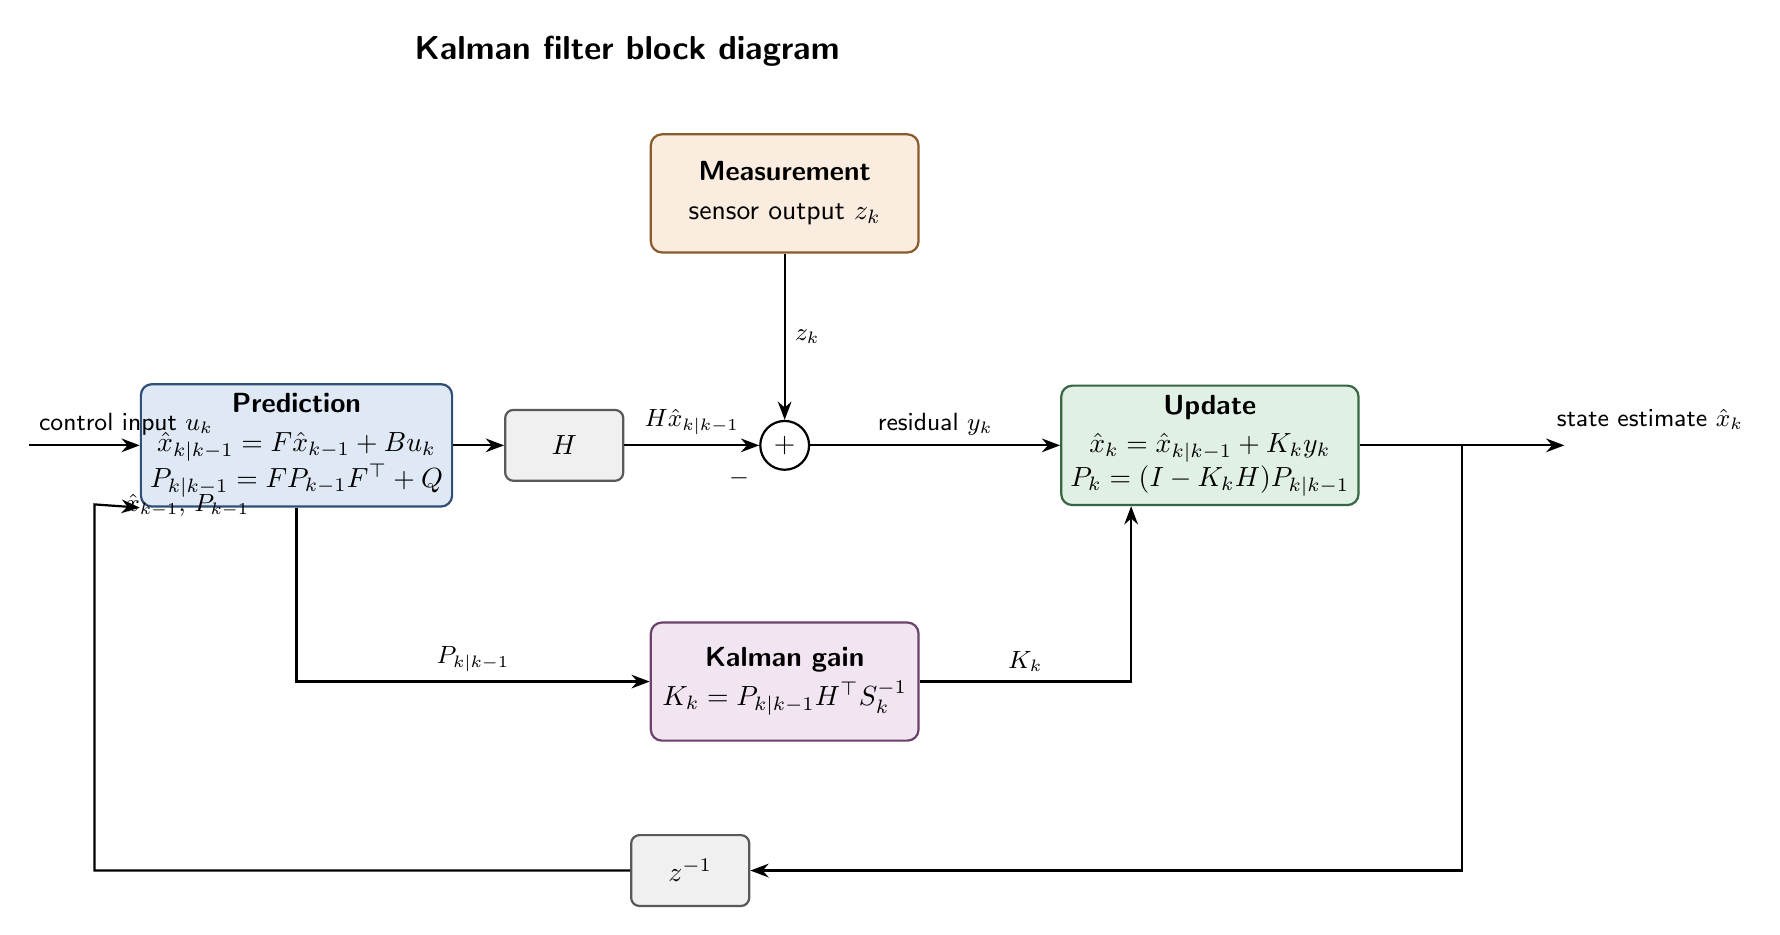
\begin{tikzpicture}[
  >=Stealth,
  font=\sffamily,
  block/.style={draw=#1!60!black,fill=#1!18,rounded corners=4pt,
    minimum width=3.4cm,minimum height=1.5cm,align=center,thick},
  small block/.style={draw=gray!70!black,fill=gray!12,rounded corners=3pt,
    minimum width=1.5cm,minimum height=0.9cm,align=center,thick},
  sum/.style={draw=black,circle,minimum size=0.62cm,inner sep=0pt,thick},
  sig/.style={->,thick},
  lab/.style={font=\small\sffamily}]

  \definecolor{predc}{RGB}{80,130,200}
  \definecolor{updc}{RGB}{90,170,110}
  \definecolor{measc}{RGB}{230,150,70}
  \definecolor{gainc}{RGB}{180,110,180}

  % blocks
  \node[block=predc] (pred) at (0,0)
    {\textbf{Prediction}\\[2pt]
     $\hat{x}_{k|k-1}=F\hat{x}_{k-1}+Bu_k$\\
     $P_{k|k-1}=FP_{k-1}F^{\top}+Q$};

  \node[block=measc] (meas) at (6.2,3.2)
    {\textbf{Measurement}\\[2pt] sensor output $z_k$};

  \node[sum] (sumres) at (6.2,0) {};
  \node at (6.2,0) {$+$};
  \node[lab] at (5.62,-0.42) {$-$};

  \node[block=gainc] (gain) at (6.2,-3.0)
    {\textbf{Kalman gain}\\[2pt]
     $K_k = P_{k|k-1}H^{\top}S_k^{-1}$};

  \node[block=updc] (upd) at (11.6,0)
    {\textbf{Update}\\[2pt]
     $\hat{x}_{k}=\hat{x}_{k|k-1}+K_k y_k$\\
     $P_{k}=(I-K_kH)P_{k|k-1}$};

  \node[small block] (delay) at (5.0,-5.4) {$z^{-1}$};

  % input
  \draw[sig] (-3.4,0) node[lab,above right] {control input $u_k$} -- (pred.west);

  % prediction to residual sum (through H)
  \node[small block] (hblk) at (3.4,0) {$H$};
  \draw[sig] (pred.east) -- (hblk.west);
  \draw[sig] (hblk.east) -- (sumres.west)
    node[lab,midway,above] {$H\hat{x}_{k|k-1}$};

  % measurement into sum
  \draw[sig] (meas.south) -- (sumres.north) node[lab,midway,right] {$z_k$};

  % residual to update
  \draw[sig] (sumres.east) -- (upd.west)
    node[lab,midway,above] {residual $y_k$};

  % gain into update (weight on residual)
  \draw[sig] (gain.east) -| ([xshift=-1.0cm]upd.south)
    node[lab,pos=0.25,above] {$K_k$};

  % prediction covariance into gain
  \draw[sig] (pred.south) |- (gain.west)
    node[lab,pos=0.75,above] {$P_{k|k-1}$};

  % update output
  \draw[sig] (upd.east) -- ++(2.6,0)
    node[lab,above left=2pt and -2.4cm] {state estimate $\hat{x}_k$};

  % feedback through unit delay back to prediction
  \draw[sig] ([xshift=1.3cm]upd.east) -- ++(0,-5.4) -- (delay.east);
  \draw[sig] (delay.west) -- ++(-6.8,0) -- ++(0,4.65) -- (pred.south west)
    node[lab,pos=0.45,right] {$\hat{x}_{k-1},\,P_{k-1}$};

  % title
  \node[font=\sffamily\bfseries\large] at (4.2,5.0) {Kalman filter block diagram};
\end{tikzpicture}
\end{document}
